
\section{Push-Pull Block Puzzles are NP-hard}
\label{2DNPhard}
In this section we show NP-hardness for Push-$k$ Pull-$l$ in 2D with thin walls for all positive integers $k$, $l$ in Section~\ref{2DNPhard} and Push-$q$ Pull-$r$ in 3D for all positive integers $q, r$ in Section~\ref{3DNPhard}. 

Thin walls are a new, but natural, notion for block pushing puzzles. They prevent blocks or the robot from passing between two adjacent, empty squares, as though there were a thin wall blocking the path. We will prove hardness by a reduction from 3SAT. The 3SAT problem asks whether, given a set of variables $\{x_1, x_2, \ldots x_n\}$ and a boolean formula in conjunctive normal form with exactly three variables per clause, there exists an assignment of values to those variables that satisfies the formula\cite{NPBook}. To do so we will introduce an abstract gadget called the Set-Verify gadget. This gadget will then be used to construct crossover gadgets (in Appendix~\ref{sec:NPCrossover}), and variable and clause gadgets.

\subsubsection{Set-Verify Gadgets}
\label{sec:SetVerifyGadgets}
The Set-Verify gadget is an abstract gadget for motion planning problems. The gadget has four entrances/exits which have different allowable paths between them depending on the state of the gadget. There are four possible states of the Set-Verify gadget: Broken, Unset, Set, and Verified. The three relevant states are depicted in Figures~\ref{setVerifyDiagrams} and \ref{SetVerifyStateTransition}. Entrances to the gadget are labeled $S_i, S_o, V_i, V_o$ and the directed arrows show the allowed passages in the shown state. Further details are given in Appendix~\ref{sec:NPCrossover}.

Since the Set-Verify gadget has no hallways with length greater than $3$, any capabilities the robot may have of pushing or pulling more than one block at a time are irrelevant. Thus, the following proof will apply for all positive values of $j$ and $k$ in Push-$j$ Pull-$k$.

\begin{figure}[!ht]
  \centering
    \begin{subfigure}[b]{0.3\textwidth}
    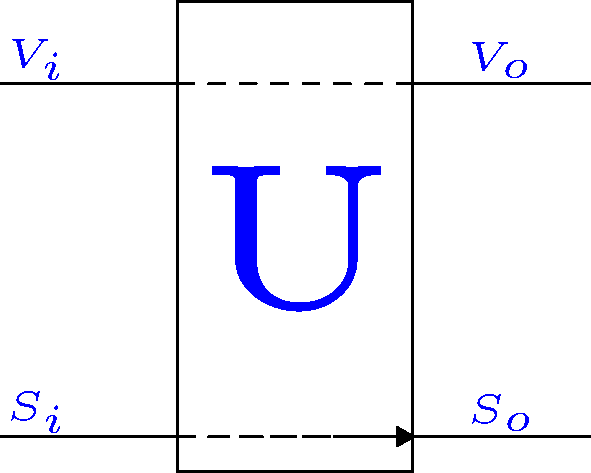
\includegraphics[width=\textwidth]{AbstractSetVerifyUnset}
    \caption{Abstract Unset Set-Verify}
    \vspace{15pt}
    \end{subfigure}
    \hfill
    \begin{subfigure}[b]{0.3\textwidth}
    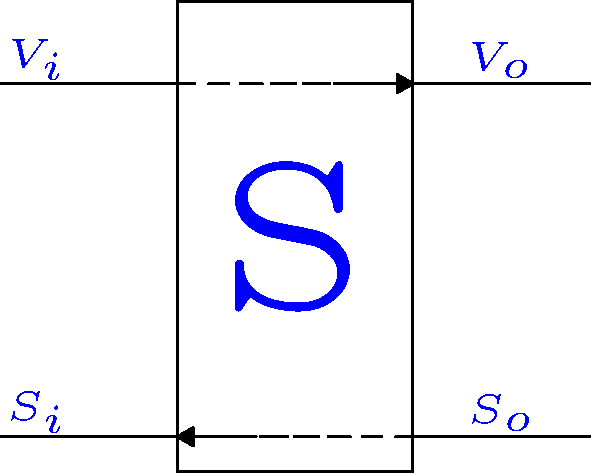
\includegraphics[width=\textwidth]{AbstractSetVerifySet}
    \caption{Abstract Set Set-Verify}
    \vspace{15pt}
    \end{subfigure}
    \hfill
    \begin{subfigure}[b]{0.33\textwidth}
    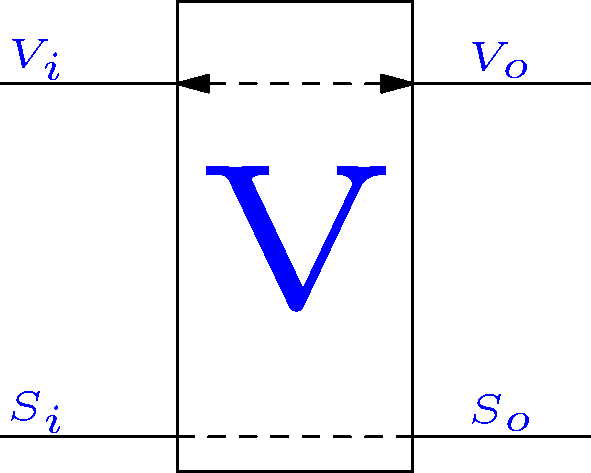
\includegraphics[width=.9\textwidth]{AbstractSetVerifyVerified}
    \caption{Abstract Verified Set-Verify}
    \vspace{15pt}
  \end{subfigure}  
   \vspace{10pt}
  \begin{subfigure}[b]{0.3\textwidth}
    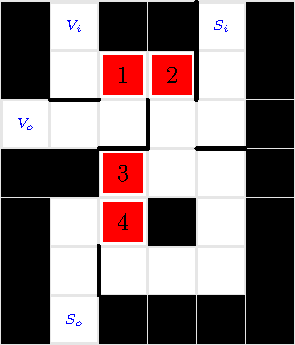
\includegraphics[width=\textwidth]{SetVerifyUnset}
    \caption{Set-Verify, unset state}
    \label{SetVerifyUnset}
  \end{subfigure}
  \hfill
  \begin{subfigure}[b]{0.3\textwidth}
    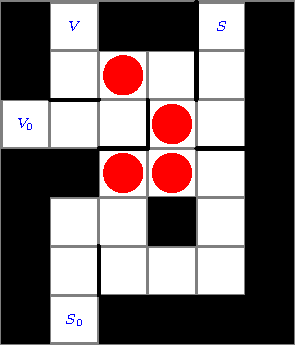
\includegraphics[width=\textwidth]{SetVerifySet}
    \caption{Set-Verify, set state}
    \label{SetVerifySet}
  \end{subfigure}
  \hfill
  \begin{subfigure}[b]{0.3\textwidth}
    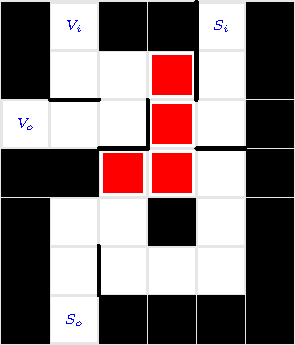
\includegraphics[width=\textwidth]{SetVerifyVerified}
    \caption{Set-Verify, verified state}
    \label{SetVerifyVerified}
  \end{subfigure}
  \caption{Diagrams of three of the states of Set-Verify gadgets along with their construction in a push-pull block puzzle. Red blocks are moveable, black blocks are fixed, thick black lines are thin walls.}
  \label{setVerifyDiagrams}
\end{figure}


\begin{table}
\begin{minipage}{.3\textwidth}
{\setlength\tabcolsep{4pt}
\begin{tabular}{>{$} l <{$} >{$} l <{$} >{$} l <{$} >{$} l <{$}}
   U: & & & \\
   &(U, s_i)& \rightarrow& (S, S_o) \\
\end{tabular}}
\end{minipage}
\begin{minipage}{.3\textwidth}
{\setlength\tabcolsep{4pt}
\begin{tabular}{>{$} l <{$} >{$} l <{$} >{$} l <{$} >{$} l <{$}}
  S: & & & \\
   &(S, s_o)& \rightarrow& (U, S_i) \\
   &(S, v_i)& \rightarrow& (V, v_o) \\
\end{tabular}}
\end{minipage}  
\begin{minipage}{.3\textwidth}
{\setlength\tabcolsep{4pt}
\begin{tabular}{>{$} l <{$} >{$} l <{$} >{$} l <{$} >{$} l <{$}}
   V: & & & \\
   &(V, v_i)& \rightarrow& (V, v_o) \\ 
   &(V, v_o)& \rightarrow& (V, v_i) \\ 
   &(V, v_o)& \rightarrow& (S, v_i) \\ 
\end{tabular}}
\end{minipage}
\caption{State transitions of a Set-Verify gadget as seen in Figure~\ref{setVerifyDiagrams}}
\label{SetVerifyStateTransition}
\end{table}

\subsubsection{Variable and Clause Gadgets}
\label{sec:2DPushPull3SAT}

We will be making use of the Set-Verify gadget to produce the literals in our 3SAT formula. One significant difficulty with this model is the complete reversibility of all actions. Thus we need to take care to ensure that going backward at any point does not allow the robot to cheat in solving our 3SAT instance. The directional properties of the Set-Verify allow us to create sections where we know if the robot exits, it must have either reset everything to the initial configuration or have correctly proceeded through that gadget.

Our literals will be represented by Set-Verify gadgets. They are considered true when the $V_i$ to $V_o$ traversal is possible, and false otherwise. Thus we can set literals to true by allowing the robot to run through the $S_i$ to $S_o$ passage of the gadget. This allows a simple clause gadget, shown in Figure~\ref{fig:NPClauseGadget}, consisting of splitting the path into three hallways, each with the corresponding verify side of our literal. We can then pass through if any of the literals are set to true, and cannot pass otherwise. Notice that the Unset and Set states do not have a backward transition. Thus the only way to go back through the clause is through the verified literal, after which the clause has been reset to the state it was in before the robot went through it.

The variables will be encoded by a series of passages which split to allow either the true or negated literals to be set, shown in Figure~\ref{fig:NPVariableGadget}. Once the robot has gone through at least one gadget in one hallway, there are only two possibilities remaining: either the robot can continue down the hall setting more literals to true, or the robot can go back through the gadget it has just exited, returning it to its unset state. Thus, before entering or after exiting a hallway all of the literals in that hallway will be in the same state. Additionally, unset gadgets do not allow a transition from $S_o$ to $S_i$, which means at any point while setting variables, if the robot decides to go back it can only return through a hallway which has been switched to the set state. Going back through these returns them to the unset state, putting that variable gadget back in its initial configuration before the robot interacted with it.

\begin{theorem}
\label{thm:2DNPhard}
Push-$k$ Pull-$l$ in 2D with thin walls is NP-hard.
\end{theorem}
\begin{proof}
    We will reduce from 3SAT. Given a 3SAT instance with variables $(x_1, x_2, \ldots x_n)$ and clauses $(x_a, x_b, \overline x_c), \ldots$, we will construct an equivalent PushPull instance as follows: 

    First, we will set up the clause gadgets. Each clause gadget will look like Figure~\ref{fig:NPClauseGadget}, with all of the Set-Verify gadgets initially in the unset state. There will be one clause gadget for each clause in the 3SAT formula. The clauses will be linked together in series, $C_k$ $out$ to $C_{k+1}$ in. At the final clause gadget's exit, we will place the goal square.

    Next, we will set up the variable gadgets. For each variable $x_k$, there will be a variable gadget $X_k$, consisting of a positive literal pathway, connecting to every clause where the variable is used positively, and a negative literal pathway, connecting to every clause where the variable is negated, as shown in Figure~\ref{fig:NPVariableGadget}. These variable gadgets will be linked together in series, $X_k$ $out$ to $X_{k+1}$ $in$. The final variable gadget's $out$ exit will be linked to the first clause gadget's $in$. Just in front of the first variable gadget's $in$ entrance will be the start square.

    The connections between these gadgets will consist of empty hallways, except where such hallways would cross. The hallways inside the clause and variable gadgets will also need to cross, and we will handle them similarly. We need crossovers for this reduction, rather than reducing to a PlanarSAT variant, because we need crossovers just to make the clause gadgets work.
    
    At all crossings, we will place a Two Use Directed Crossover, from Figure~\ref{fig:OneUseCrossover}. The orientation of the gadget will be chosen according to a specified ordering, where the later pathway will never be used before the earlier pathway, and no pathway will every be traversed twice in the same direction. The ordering is each variable gadget's hallways, in increasing order of the variable gadgets, followed by each clause gadget's hallways, in increasing order of clause gadgets. Within the variable gadgets, the ordering will be from in to out along the positive and negative lines, with the positive lines arbitrarily placed before the negative lines. The clause gadget hallways won't cross each other.

    The construction is complete. To see that it is solvable if and only if the corresponding SAT problem is satisfiable, first let us consider the case where the SAT problem is satisfiable. If the SAT problem is satisfiable, then there is an assignment of variables such that each clause is satisfied, e.g. has at least one true literal. Therefore, the PushPull construction is solvable. It can be solved by traversing each variable gadget via the side corresponding to the satisfying assignment, then traversing each clause, which is passable because it is satisfied. The crossovers do not impede traversal, since the path taken goes through each crossover at most once of each of its pathways, and strictly in the forward direction of the ordering which determined the orientation of the crossovers. Thus, the entire PushPull problem can be solved, as desired.

    Next, let us consider the case where the SAT problem is not satisfiable. Consider a partial traversal of the PushPull problem, from the start cell through the variable gadgets. Regardless of any reverse transitions through a variable gadget or interactions with its clause gadget, if the robot is beyond a given variable gadget exactly one of the variable lines must be set and the other must be unset. Likewise, the interactions with the crossover gadgets do not allow any transitions other than within the variable gadgets, regardless of reversals. Moreover, interactions with the clause gadgets only change the state of Set-Verify gadgets corresponding to literals between the Set and Verified states. If a Set-Verify is Unset, its state cannot be altered via its verify line ($V_i - V_o$).

    Thus, regardless of the robot's prior movements, the only literals that will be Set or Verified are at most those corresponding to a single assignment for each variable. No two literals corresponding to opposite assignments of the same variable will every be in the Set or Verified states at the same time. 

    Since the SAT problem is assumed to be unsatisfiable, no assignment of variables will satisfy every clause. Thus, as the robot exits the variable gadgets and enters the clause gadgets, for any prior sequence of moves, there must be some clause gadget which has all of its literals in the Unset state, corresponding to the unsatisfied clause for this setting of variables. Since all clauses must be traversed to reach the goal cell, and a clause cannot be traversed if all of its literals are Unset, the robot cannot reach the goal cell. Thus, the PushPull problem is unsolvable.

    We have demonstrated that the PushPull problem is solvable if and only if the corresponding 3SAT instance is satisfiable. The reduction mentioned above is polynomial time reduction, as long as the hallways are constructed reasonably. Thus, Push-$k$ Pull-$l$ in 2D with thin walls is NP-hard.

\end{proof}

